%%%%%%%%%%%%%%%%%%%%%%%%%%%%%%%%%%%%%%%%%
% University/School Laboratory Report
% LaTeX Template
% Version 3.1 (25/3/14)
%
% This template has been downloaded from:
% http://www.LaTeXTemplates.com
%
% Original author:
% Linux and Unix Users Group at Virginia Tech Wiki 
% (https://vtluug.org/wiki/Example_LaTeX_chem_lab_report)
%
% License:
% CC BY-NC-SA 3.0 (http://creativecommons.org/licenses/by-nc-sa/3.0/)
%
%%%%%%%%%%%%%%%%%%%%%%%%%%%%%%%%%%%%%%%%%

%----------------------------------------------------------------------------------------
%	PACKAGES AND DOCUMENT CONFIGURATIONS
%----------------------------------------------------------------------------------------

\documentclass{article}
\usepackage[margin=.75in]{geometry}
\usepackage{hyperref}
\usepackage[version=3]{mhchem} % Package for chemical equation typesetting
\usepackage{siunitx} % Provides the \SI{}{} and \si{} command for typesetting SI units
\usepackage{graphicx} % Required for the inclusion of images
\usepackage{natbib} % Required to change bibliography style to APA
\usepackage{amsmath} % Required for some math elements 

\setlength\parindent{1em} % Removes all indentation from paragraphs
\setlength{\parskip}{1em}
\renewcommand{\labelenumi}{\alph{enumi}.} % Make numbering in the enumerate environment by letter rather than number (e.g. section 6)

%\usepackage{times} % Uncomment to use the Times New Roman font

%----------------------------------------------------------------------------------------
%	DOCUMENT INFORMATION
%----------------------------------------------------------------------------------------

\title{Weekly Catchup} % Title

\author{Weixiong Zheng} % Author name

\date{\today} % Date for the report

\begin{document}

\maketitle % Insert the title, author and date
% If you wish to include an abstract, uncomment the lines below
% \begin{abstract}
% Abstract text
% \end{abstract}

%----------------------------------------------------------------------------------------
%	SECTION 0
%----------------------------------------------------------------------------------------
\section{Updates on previous goals}
Previous goal was to give out the diagram of the existing BART so as to show what classes
we have right now.
%----------------------------------------------------------------------------------------
%	SECTION 1
%----------------------------------------------------------------------------------------
\section{Progress up to now}
Talked to Alex about his background and basics we need to get started. Gives out basic introduction materials on finite element (thanks to Josh). We might set up a time per week with a white board so I 
can either teach a bit or we can have a discussion to help Alex get started. His experience on FVM should make 
him easy to transfer to FEM.

Continuous exploration was put in how to use CTest. Besides, in order to show Josh how CTest can be used in a way similar to GTest, a unit test for {\tt ProblemDefinition} along with its rewriting was created. Specifically, {\tt AssertThrow} in {\tt deal.II} was used to mimic {\tt ASSERT\_EQ/EXPECT\_EQ} functionalities. That being said, CTest can either be used without knowing what the right output beforehand or used in a way similar to GTest by knowing what correct answers are beforehand.

Additionally, diagrams were created based on {\tt devel} branch. Figure\ \ref{f:inheritance-instantiation}\ presents the inheritance relationships of classes. Diamond shows where the classes are instantiated and arrows present the inheritance (base classes are the classes arrows pointing to).

\begin{figure}
	\centering
	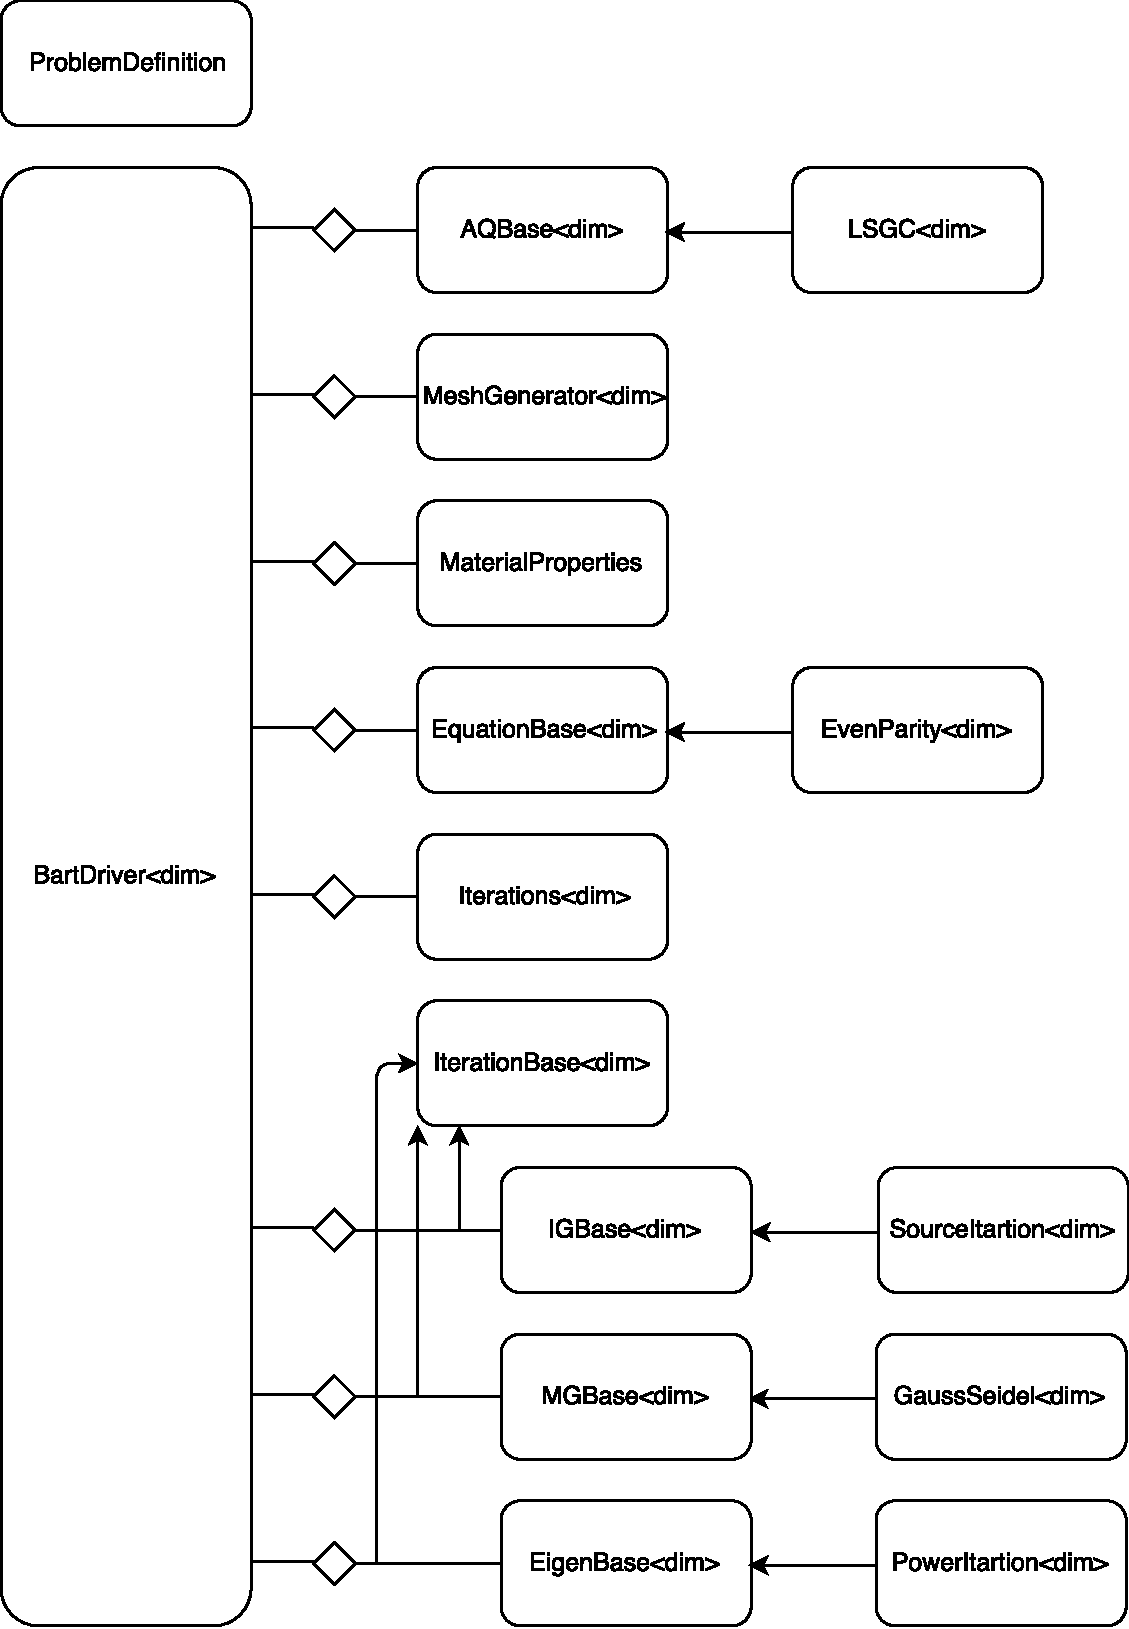
\includegraphics[scale=0.7]{pics/instantiation-inheritance}
	\caption{Inheritance and instantiation diagram.}
	\label{f:inheritance-instantiation}
\end{figure}

Figure\ \ref{f:class-usage}\ illustrates where class methods or derived class methods are actually invoked.

\begin{figure}
	\centering
	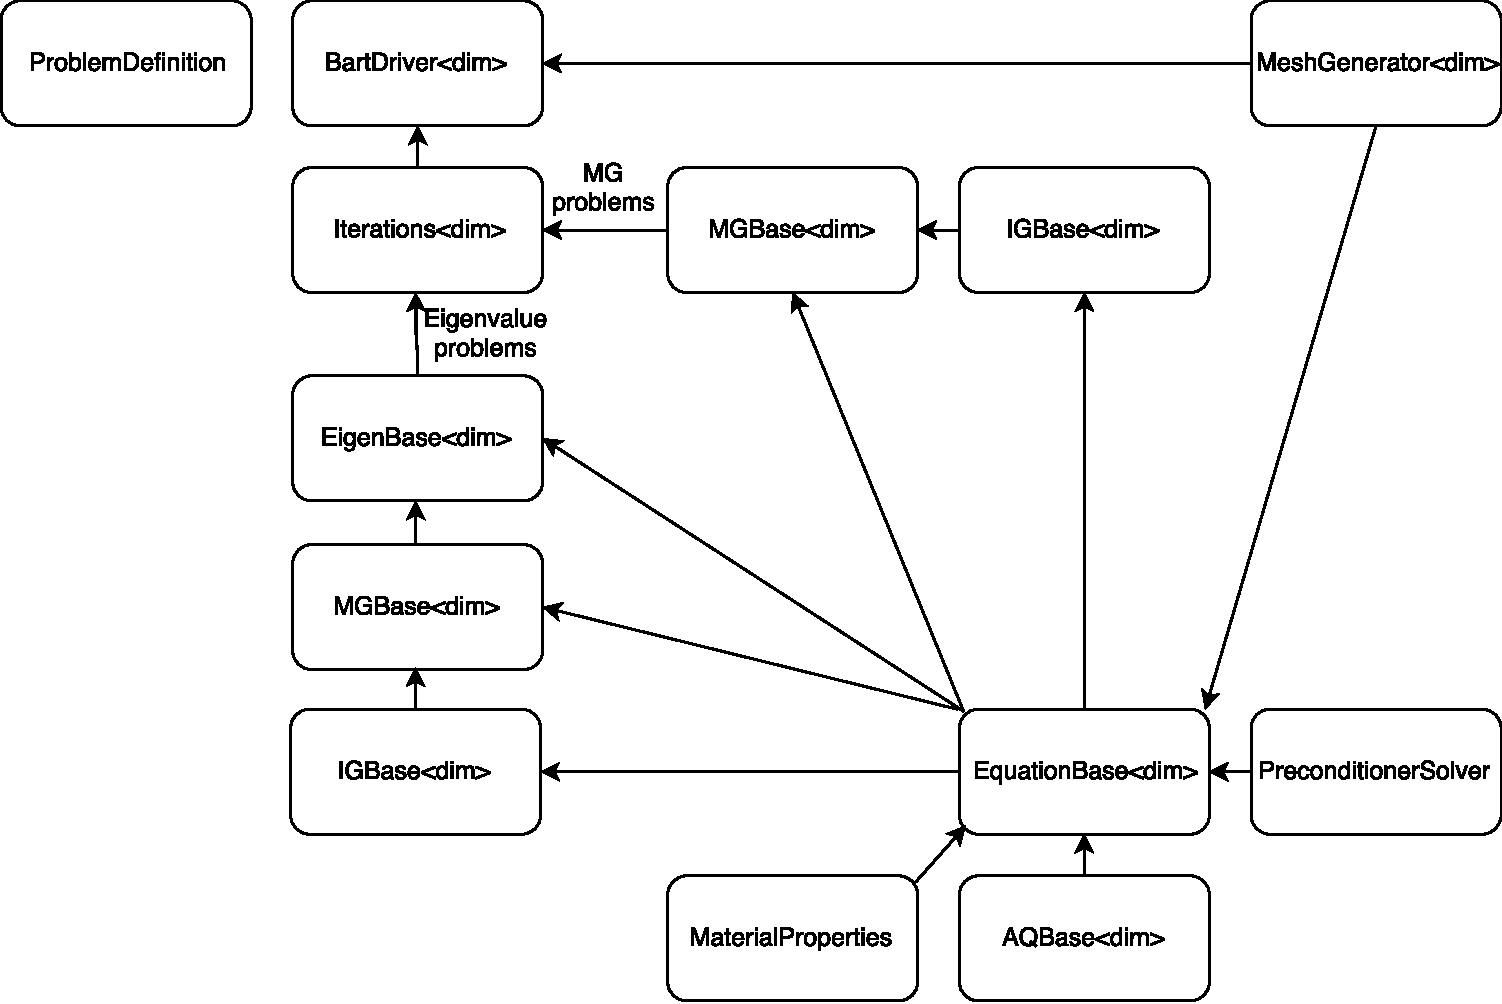
\includegraphics[scale=0.7]{pics/class-usage}
	\caption{Class usage diagram.}
	\label{f:class-usage}
\end{figure}

It would be hard to explain all the functionalities of specific class within diagrams. I'd suggest people interested refer to {\tt Doxygen} documentation of {\tt devel} branch.

Efforts were also put into setting up notifications (unfortunately because of mistakenly understanding hooks). Final resolution does not actually involve either git hooks or web hooks. 
%----------------------------------------------------------------------------------------
%	SECTION 2
%----------------------------------------------------------------------------------------
\section{Things you need from Rachel}


%----------------------------------------------------------------------------------------
%	SECTION 3
%----------------------------------------------------------------------------------------
\section{Goals/Things will be going on}
I will talk to Josh to set up a mutually acceptable fashion of doing unit test using CTest as 
our preference differentiate. Once done, I'd add it to style guide and continue the rewriting.

Josh will be trying to simplify CMakeLists.txt. The expectation is s.t. everything will be contained 
in the highest level CMakeLists.txt, in the BART folder.

%----------------------------------------------------------------------------------------
%	SECTION 4
%----------------------------------------------------------------------------------------
%\section{Links to any related materials}



%----------------------------------------------------------------------------------------
%	BIBLIOGRAPHY
%----------------------------------------------------------------------------------------

%\bibliographystyle{apalike}
%
%\bibliography{sample}

%----------------------------------------------------------------------------------------


\end{document}